\documentclass[11pt,a4paper]{article}
			\usepackage[french]{babel}
					
				\usepackage{pifont}  
				\usepackage[utf8x]{inputenc}
				\usepackage[T1]{fontenc} 
				\usepackage{lmodern}			
				\usepackage{fancyhdr}
				\usepackage{textcomp}
				\usepackage{makeidx}
				\usepackage{tabularx}
				\usepackage{multicol}
				\usepackage{multirow}
				\usepackage{longtable}
				\usepackage{color}
				\usepackage{soul}
				\usepackage{boxedminipage}
				\usepackage{shadow}
				\usepackage{framed}			
				\usepackage{array}
				\usepackage{url}
				\usepackage{ragged2e}
				\usepackage{fancybox}
				\newcommand{\cadretitre}[2]{
				  \vspace*{0.8\baselineskip}
				  \begin{center}%
				  \boxput*(0,1){%
					%\colorbox{white}{\Large\textbf{\ #1\ }}%
				  }%
				  {%
					\setlength{\fboxsep}{10pt}%
				    \Ovalbox{\begin{minipage}{.8\linewidth}\begin{center}\Large\sffamily{#2}\end{center}\end{minipage}}}%
				  \end{center}
				  \vspace*{2\baselineskip}
				  }
			
			\makeatletter
			\def\@seccntformat#1{\protect\makebox[0pt][r]{\csname the#1\endcsname\quad}}
			\makeatother

				% Permet d'afficher qqchose à une positin absolue
				\usepackage[absolute]{textpos}
				\setlength{\TPHorizModule}{1cm}
				\setlength{\TPVertModule}{\TPHorizModule}
	
				\usepackage[titles]{tocloft}
				\setlength{\cftbeforesecskip}{0.5ex}
				\setlength{\cftbeforesubsecskip}{0.2ex}
				\addto\captionsfrench{\renewcommand\contentsname{}}
				
				\usepackage[font=scriptsize]{caption}
				
				\usepackage{listings}
\lstdefinestyle{lstverb}
  {
    basicstyle=\footnotesize,
    frameround=tttt, frame=trbl, framerule=0pt, rulecolor=\color{gray},
    lineskip=-1pt,   % pour rapprocher les lignes
    flexiblecolumns, escapechar=\\,
    tabsize=4, extendedchars=true
  }
\lstnewenvironment{Java}[1][]{\lstset{style=lstverb,language=java,#1}}{}
				\ifx\pdfoutput\undefined
					\usepackage{graphicx}
				\else
					\usepackage[pdftex]{graphicx}
				\fi
				\usepackage[a4paper, hyperfigures=true, colorlinks, linkcolor=black, citecolor=blue,urlcolor=blue, pagebackref=true, bookmarks=true, bookmarksopen=true,bookmarksnumbered=true,
                pdfauthor={}, pdftitle={TD Séquentiel - Rappels de base}, pdfkeywords={TD S\'equentiel - Rappels de base, },pdfpagemode=UseOutlines,pdfpagetransition=Dissolve,nesting=true,
				backref, pdffitwindow=true, bookmarksnumbered=true]{hyperref}
				\usepackage{supertabular}
				\usepackage[table]{xcolor}
				\usepackage{url}
				\usepackage{caption} 
				\setlength{\parskip}{1.3ex plus 0.2ex minus 0.2ex}
				\setlength{\parindent}{0pt}
				
				\makeatletter
				\def\url@leostyle{ \@ifundefined{selectfont}{\def\UrlFont{\sf}}{\def\UrlFont{\footnotesize\ttfamily}}}
				\makeatother
				\urlstyle{leo}
				
				\definecolor{examplecolor}{rgb}{0.156,0.333,0.443}
				\definecolor{definitioncolor}{rgb}{0.709,0.784,0.454}
				\definecolor{exercisecolor}{rgb}{0.49,0.639,0}
				\definecolor{hintcolor}{rgb}{0.941,0.674,0.196}
				\definecolor{tableHeadercolor}{rgb}{0.709,0.784,0.454}
				\definecolor{tablerowAltcolor}{rgb}{.866,.905,.737}
				\definecolor{tablerowAlt2color}{rgb}{.968,.976,.933}
				\definecolor{verylightgray}{rgb}{0.98,0.98,0.98}
				
				\newenvironment{fshaded}{
				\def\FrameCommand{\fcolorbox{framecolor}{shadecolor}}
				\MakeFramed {\FrameRestore}}
				{\endMakeFramed}
				
				\newenvironment{fexample}[1][]{\definecolor{shadecolor}{rgb}{.913,.913,.913}
				\definecolor{framecolor}{rgb}{.156,.333,.443}
				\begin{fshaded}}{\end{fshaded}} 
				
				\newenvironment{fdefinition}{\definecolor{shadecolor}{rgb}{.913,.913,.913}
				\definecolor{framecolor}{rgb}{.709,.784,.454}
				\begin{fshaded}}{\end{fshaded}}
				
				\newenvironment{fexercise}{\definecolor{shadecolor}{rgb}{.913,.913,.913}
				\definecolor{framecolor}{rgb}{.49,.639,0}
				\begin{fshaded}}{\end{fshaded}}
				
				\newenvironment{fhint}{\definecolor{shadecolor}{rgb}{.913,.913,.913}
				\definecolor{framecolor}{rgb}{.941,.674,.196}
				\begin{fshaded}}{\end{fshaded}}	
				
				\newcommand{\PreserveBackslash}[1]{
				\let\temp=\\#1\let\\=\temp
				}
				\let\PBS=\PreserveBackslash
				\newcolumntype{A}{>{\PBS\raggedright\small\hspace{0pt}}X}
				\newcolumntype{L}[1]{>{\PBS\raggedright\small\hspace{0pt}}p{#1}}
				\newcolumntype{R}[1]{>{\PBS\raggedleft\small\hspace{0pt}}p{#1}}
				\newcolumntype{C}[1]{>{\PBS\centering\small\hspace{0pt}}p{#1}}
				
				\makeindex
				
				\title{TD S\'equentiel - Rappels de base}	
			\date{}
			\author{\scriptsize{}}
			\definecolor{light-gray}{gray}{0.8}
			\renewcommand{\headrulewidth}{0pt}
			\fancyhead[L]{
				\footnotesize\textsc{Haute \'Ecole de Bruxelles}\\
	    			\footnotesize\textsc{\'Ecole Sup\'erieure d'Informatique}
			}
			\fancyhead[R]{
				\footnotesize{Bachelor en Informatique}\\
				\footnotesize{Laboratoires Java} - 
			\footnotesize{1\`ere ann\'ee}}
				\fancyfoot[L]{ }
				\fancyfoot[C]{}
				\fancyfoot[R]{\scriptsize{\textcolor{gray}{version 2014-2015 (\today)}}}
				\pagestyle{plain}
				\reversemarginpar
				\usepackage{rotating}						
				\begin{document}
					\begin{textblock}{9}(2,3.2)
						
\includegraphics[width=2cm]{../../../_templates/java/icons/logo-esi}
					\end{textblock}
				
				
				
				
				%\maketitle
				\cadretitre{TD1}{TD S\'equentiel - Rappels de base}
				\thispagestyle{fancy}
        \marginpar{\begin{sideways}
            \begin{minipage}[t]{1cm}
            \begin{tiny}
            
\includegraphics[width=1\linewidth,height=1\textheight,keepaspectratio=true]{../../../_templates/java/icons/cc-gris.jpg}
			\end{tiny}
			\end{minipage}
            \begin{minipage}[b]{19cm}
            \begin{tiny}
            \textcolor{gray}{Distribué sous licence Creative Commons Paternité - Partage à l'Identique 2.0 Belgique 
            (\texttt{http://creativecommons.org/licenses/by-sa/2.0/be/})
			\vspace{-1em}
			\\Les autorisations au-delà du champ de cette licence peuvent être obtenues à 
			\texttt{http://www.heb.be/esi}
			- \texttt{mcodutti@heb.be}
			}\end{tiny}
			\end{minipage}
        \end{sideways}}
            \begin{abstract}
			Ce TD a pour but de fixer les bases du LDA et de la programmation Java.
		
            \par
        \end{abstract}
				\vspace{-2em}\tableofcontents
				\pagestyle{plain}
            \clearpage
            \fancyhead[L,C,R]{}
            \fancyfoot[L,C]{}
            \fancyfoot[R]{ \scriptsize{\textcolor{gray}{
				TDSeq - page \thepage}}}
				\thispagestyle{fancy}
				\pagestyle{fancy}
	   
            \section{Algorithmes s\'equentiels}Revoyons ici les bases du pseudo-code et leur traduction en Java.\subsection{Le pseudo-code}
		    Le pseudo-code ou Langage de Description des Algorithmes (LDA en abr\'eg\'e) est un langage
        formel et symbolique utilisant :
        
					\begin{itemize}
				
			\item 
            des noms symboliques destin\'es \`a repr\'esenter les objets sur lesquels s'effectuent des
            actions ;
          
			\item 
            des op\'erateurs symboliques ou des mots-cl\'es traduisant les op\'erations primitives
            ex\'ecutables par un ex\'ecutant donn\'e ;
          
			\item 
            des structures de contr\^ole types.
          
					\end{itemize}
				
            \par
        \section{Variables et types}
				Nous savons que les op\'erations que l'ordinateur devra ex\'ecuter portent sur des \'el\'ements qui
        sont les \textbf{donn\'ees} du probl\`eme.
      
            \par
        
        Lorsqu'on attribue un \textbf{nom} 
        et un \textbf{type} \`a ces donn\'ees, on
        parle alors de \textbf{variables}. 
      
            \par
        
        Dans un algorithme, une variable conserve toujours son nom et
        son type, mais peut changer de \textbf{valeur}.
         
					\begin{itemize}
				
			\item 
            Le \textbf{nom} d'une variable permet de la caract\'eriser et de la reconnaitre ;
          
			\item 
            le \textbf{type} d'une variable d\'ecrit la nature de son contenu.
          
					\end{itemize}
				
            \par
        \subsection{Les types autoris\'es en algo}
          Dans un premier temps, les seuls types utilis\'es sont :
          
					\begin{itemize}
				
			\item \verb@entier@ pour les nombres entiers ;
			\item \verb@réel@ pour les nombres r\'eels ;
			\item \verb@caractère@ pour les diff\'erentes lettres et caract\`eres
              (par exemple ceux qui apparaissent sur un clavier : 'a', '1', '\#', etc.)
			\item \verb@chaine@ pour les variables contenant un ou plusieurs caract\`ere(s) ou aucun (la chaine vide)
              (par exemple : "Bonjour", "Bonjour le monde", "a", "", etc.)
			\item \verb@booléen@ les variables de ce type 
            ne peuvent valoir que \verb@vrai@ ou \verb@faux@
					\end{itemize}
				
            \par
        
			
		\subparagraph{Le type des donn\'ees} 
		
                \textcolor{white}{.} \par
             
								Quel(s) type(s) de donn\'ees utiliseriez-vous pour repr\'esenter :
							
					\begin{itemize}
				
			\item un prix hors tva ? \textcolor{gray}{\underline{\hspace*{3em}}} 
			\item votre nom ?  \textcolor{gray}{\underline{\hspace*{5em}}} 
			\item vos initiales ? \textcolor{gray}{\underline{\hspace*{10em}}} 
			\item la longueur d'un rectangle ?  \textcolor{gray}{\underline{\hspace*{3em}}} 
			\item une date du calendrier ?  \textcolor{gray}{\underline{\hspace*{10em}}} 
			\item un moment dans la journ\'ee ?  \textcolor{gray}{\underline{\hspace*{10em}}} 
					\end{itemize}
				\subsection{Les types \'equivalents en java}
          Les \'equivalents Java des types donn\'es en algo sont
          
					\begin{itemize}
				
			\item \verb@int@ pour le type \verb@entier@ pour les nombres entiers ;
			\item \verb@double@ pour le type \verb@réel@ pour les nombres r\'eels ;
			\item \verb@char@ pour le type \verb@caractère@ pour les diff\'erentes lettres et caract\`eres
			\item \verb@String@ pour le type \verb@chaine@ 
              pour les variables contenant un ou plusieurs caract\`ere(s) ou aucun (la chaine vide)
            
			\item \verb@boolean@ pour le type \verb@booléen@ les variables de ce type 
            ne peuvent valoir, en Java, que \verb@true@ ou \verb@false@
					\end{itemize}
				
            \par
        
			
		\subparagraph{Les commandes de base} 
		
                \textcolor{white}{.} \par
             
								Quel(s) type(s) de donn\'ees utiliseriez-vous pour repr\'esenter :
							
					\begin{itemize}
				
			\item un prix hors tva ? \textcolor{gray}{\underline{\hspace*{5em}}} 
			\item votre nom ?  \textcolor{gray}{\underline{\hspace*{5em}}} 
			\item une de vos initiales ? \textcolor{gray}{\underline{\hspace*{3em}}} 
			\item la longueur d'un rectangle ?  \textcolor{gray}{\underline{\hspace*{5em}}} 
			\item le jour d'une date du calendrier ?  \textcolor{gray}{\underline{\hspace*{2em}}} 
			\item les heures d'un moment dans la journ\'ee ?  \textcolor{gray}{\underline{\hspace*{2em}}} 
					\end{itemize}
				\subsection{Java est un langage fortement typ\'e.}
			    Java est un langage fortement typ\'e.
			  
            \par
        
          Toute donn\'ee a un type. Quels types ?
          
					\begin{itemize}
				
			\item \verb@primitifs prédéfinis : @ entier, r\'eel, bool\'een (logique) ;
			\item \verb@références prédéfinis :@ tableaux, String, . . . ;
			\item \verb@références définis par le programmeur@
					\end{itemize}
				
            \par
        
			
		\subparagraph{Les types primitifs} 
		
					\textcolor{white}{.} \par
				
            \par
        \begin{figure}[hbt]
				    \begin{center}
					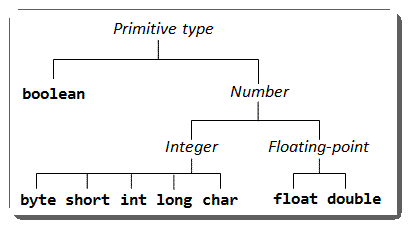
\includegraphics[width=0.8\linewidth,height=0.8\textheight,keepaspectratio=true]{/home/clr/Documents/Cours/DEV1Q2/TDSeq/fr/image/primitifs.png}
						\end{center}
                
                    \caption[primitifs.png]{primitifs.png}
                \end{figure}
                    
            \par
        
			
		\subparagraph{Les types primitifs num\'eriques entiers} 
		
					\textcolor{white}{.} \par
				
            \par
        
          Les types primitifs num\'eriques entiers sont
          \verb@byte@, \verb@short@, 
          \verb@int@ et \verb@long@ (\verb@char@ sera vu \`a part),
          
					\begin{itemize}
				
			\item  ce sont des nombres sign\'es (en compl\'ement \`a 2)
			\item  ils sont cod\'es sur 
              
					\begin{itemize}
				
			\item  8 bits pour un \verb@byte@ ;
			\item  16 bits pour un \verb@short@ ;
			\item  32 bits pour un \verb@int@ ;
			\item  64 bits pour un \verb@long@ ;
					\end{itemize}
				
			\item  ils comprennent donc les valeurs :
              
					\begin{itemize}
				
			\item  -128 \`a 127 pour un \verb@byte@ ;
			\item  -32768 \`a 32767 pour un \verb@short@ ;
			\item  -2147483648 \`a 2147483647 pour un \verb@int@ ;
			\item  -9223372036854775808 \`a 9223372036854775807 pour un \verb@long@ ;
					\end{itemize}
				
					\end{itemize}
				
            \par
        
			
		\subparagraph{Les litt\'eraux pour les types primitifs num\'eriques entiers} 
		
					\textcolor{white}{.} \par
				
            \par
        
          Un \textbf{litt\'eral}, c'est une notation pour repr\'esenter une valeur fix\'ee directement dans un code  source.
        
            \par
        
          Un \textbf{litt\'eral num\'erique d\'ecimal} est
            
					\begin{itemize}
				
			\item une suite de chiffres
			\item \'eventuellement s\'epar\'es par\,\verb|_|\, pour la lisibilit\'e
			\item suivi \'eventuellement du suffixe ( \,\verb|l|\, ou \,\verb|L|\,) 
                qui distingue un \verb@int@ d'un \verb@long@
			\item pas de \verb@byte@ ou \verb@short@, 
                un litt\'eral est \verb@int@ (ou \verb@long@)
					\end{itemize}
				
            \par
        
          Un \textbf{litt\'eral num\'erique octal} est
            
					\begin{itemize}
				
			\item une suite de chiffres de 0 \`a 7
			\item pr\'ec\'ed\'e de 0.
					\end{itemize}
				
            \par
        
          Un \textbf{litt\'eral num\'erique hexad\'ecimal} est
            
					\begin{itemize}
				
			\item une suite de chiffres et lettres a,b,c,d,e,f (minuscules/majuscules)
			\item pr\'ec\'ed\'e de 0x ou 0X
					\end{itemize}
				
            \par
        
          Un \textbf{litt\'eral num\'erique binaire} est
            
					\begin{itemize}
				
			\item une suite de chiffres 0 et 1
			\item pr\'ec\'ed\'e de 0b ou 0B
					\end{itemize}
				
            \par
        
          Par exemple, la quantit\'e 100 de type \verb@int@ peut s'\'ecrire 
            
					\begin{itemize}
				
			\item 100
			\item 1\_0\_0
			\item 0144
			\item 01\_44
			\item 0x64
			\item 0b110\_0100
					\end{itemize}
				
            \par
        
			
		\subparagraph{Le type num\'erique caract\`ere} 
		
					\textcolor{white}{.} \par
				
            \par
        \verb@char@ est
          
					\begin{itemize}
				
			\item un caract\`ere Unicode cod\'e en UTF16
			\item un entier non sign\'e sur 16 bits
			\item assimil\'e \`a un entier 
					\end{itemize}
				
            \par
        
          Pour un litt\'eral de type char : un caract\`ere entre single quote.
          Par exemple : 'a', '1', ' ', ...
        
            \par
        
          Il existe des s\'equences d'\'echappement pour repr\'esenter certains caract\`eres sp\'eciaux :
          
					\begin{itemize}
				
			\item \verb@\n@ pour repr\'esenter un \textbf{saut de ligne}
			\item \verb@\t@ pour repr\'esenter une \textbf{tabulation}
			\item \verb@\'@ pour repr\'esenter le caract\`ere \textbf{'}
			\item \verb@\"@ pour repr\'esenter le caract\`ere \textbf{"}
					\end{itemize}
				
            \par
        
			
		\subparagraph{Les types primitifs num\'eriques flottants} 
		
					\textcolor{white}{.} \par
				
            \par
        
          Les types primitifs num\'eriques flottants sont
          \verb@float@ et \verb@double@.
          
					\begin{itemize}
				
			\item ils respectent la norme IEEE754 ;
			\item  ils sont cod\'es sur 
              
					\begin{itemize}
				
			\item  32 bits pour un \verb@float@ ;
			\item  64 bits pour un \verb@double@ ;
					\end{itemize}
				
			\item on utilisera plus souvent le type \verb@double@ ;
			\item il s'agit d'une \textbf{mod\'elisation} de la notion math\'ematique.
					\end{itemize}
				
            \par
        
			
		\subparagraph{Les litt\'eraux pour les types primitifs num\'eriques flottants} 
		
					\textcolor{white}{.} \par
				
            \par
        
          Un \textbf{litt\'eral}, c'est une notation pour repr\'esenter une valeur fix\'ee directement dans un code  source.
        
            \par
        
          Un \textbf{litt\'eral num\'erique flottant se compose de parties optionnelles (mais pas ensemble)} :
            
					\begin{enumerate}
				
			\item une partie enti\`ere
			\item .
			\item partie d\'ecimale
			\item E ou e
			\item exposant
			\item suffixe (en l'absence de suffixe : un double)
					\end{enumerate}
				
            \par
        
          Par exemple : 1.2E3, 1.F, .1, 1e−2d, 1f
        
            \par
        
          Par contre : 1, .E1, E1 ne sont pas des litt\'eraux pour les types primitifs num\'eriques flottants
        
            \par
        
			
		\subparagraph{Le type primitif bool\'een} 
		
					\textcolor{white}{.} \par
				
            \par
        \verb@boolean@
					\begin{itemize}
				
			\item aussi appel\'e logique ; 
			\item  il peut prendre 2 valeurs :
              
					\begin{itemize}
				
			\item \verb@true@ ;
			\item \verb@false@ ;
					\end{itemize}
				
			\item il prend 1 octet en m\'emoire.
					\end{itemize}
				
            \par
        
			
		\subparagraph{Les types r\'ef\'erences pr\'ed\'efinis : les chaines de caract\`eres} 
		
					\textcolor{white}{.} \par
				
            \par
        \verb@String@
					\begin{itemize}
				
			\item il s'agit de caract\`eres entre double quote : par exemple : "Java", "Bonjour tout le monde", "a",...  ; 
			\item est un type r\'ef\'erence pr\'ed\'efini ;
			\item  Attention \verb@char@ ≠ \verb@String@
					\end{itemize}
				
            \par
        \subsection{D\'eclaration de variables en algo}
          La \textbf{d\'eclaration} d'une variable est l'instruction qui d\'efinit son \textbf{nom} 
          et son \textbf{type}.
        
            \par
        \,\verb|num1, num2 : entiers|\,
            \par
        
          L'ensemble des instructions de la forme \,\verb|variable1, variable2,. . . : type|\,
          forme la partie d'un algorithme nomm\'ee \textbf{d\'eclaration des variables}. 
        
            \par
        
          La d\'eclaration des informations apparaitra toujours en \textbf{d\'ebut} d'algorithme, ou dans un bloc annexe appel\'e
          dictionnaire des variables ou encore dictionnaire des donn\'ees.
        
            \par
        
			
		\subparagraph{Valeur initiale ?} 
		
					\textcolor{white}{.} \par
				
            \par
        
          Attention, lors de la d\'eclaration d'une variable, \textbf{celle-ci n'a pas de valeur} ! 
          Nous verrons que c'est l'instruction d'affectation qui va servir \`a donner un contenu aux variables d\'eclar\'ees.
        
            \par
        
			
		\subparagraph{Comment nommer correctement une variable ?} 
		
					\textcolor{white}{.} \par
				
            \par
        
          Le but est de trouver un nom qui soit suffisamment \textbf{court}, 
          tout en restant \textbf{explicite} et ne pr\^etant \textbf{pas \`a confusion}.
        
            \par
        
          Ainsi \textit{num1} est plus appropri\'e pour d\'esigner le premier num\'erateur 
          que \textit{zozo1}, \textit{tintin}, \textit{bidule}
          ou \textit{premierNum\'erateur}. 
          De m\^eme, ne pas appeler \textit{den} la variable repr\'esentant le num\'erateur.
        
            \par
        
          Il faut aussi tenir compte que les langages de programmation imposent certaines limitations
          (parfois diff\'erentes d'un langage \`a l'autre) ce qui peut n\'ecessiter une modification du nom
          lors de la traduction.
        
            \par
        
          Voici quelques r\`egles et limitations traditionnelles dans les langages de programmation :
          
					\begin{itemize}
				
			\item 
            Un nom de variable est g\'en\'eralement une suite de caract\`eres alphanum\'eriques d'un
            seul tenant (pas de caract\`eres blancs) et ne commen\c cant jamais par un chiffre. Ainsi
            x1 est correct mais pas 1x.
            
			\item 
            Pour donner un nom compos\'e \`a une variable, on peut utiliser le \guillemotleft  tiret bas \guillemotright  ou underscore 
            (par ex. premier\_num\'erateur) mais on d\'econseille d'utiliser le signe \guillemotleft  - \guillemotright  qui est
            plut\^ot r\'eserv\'e \`a la soustraction. Ainsi, dans la plupart des langages, premier-num\'erateur
            serait interpr\'et\'e comme la soustraction des variables premier et num\'erateur.
            
			\item 
            Une alternative \`a l'utilisation du tiret bas pour l'\'ecriture de noms de variables compos\'es
            est la notation \guillemotleft  chameau \guillemotright  (camelCase en anglais), qui consiste \`a mettre une majuscule
            au d\'ebut des mots (g\'en\'eralement \`a partir du deuxi\`eme), par exemple premierNombre
            ou dateNaissance.
            
			\item 
            Les indices et exposants sont proscrits.
            
			\item 
            Les mots-cl\'es du langage sont interdits (par exemple for, if, while pour Java et Cobol)
            et on d\'econseille d'utiliser les mots-cl\'es du pseudo-code (tels que Lire, Afficher, pour. . .)
            
			\item 
            Certains langages n'autorisent pas les caract\`eres accentu\'es (tels que \`a, \c c, \^e, \o, etc.)
            ou les lettres des alphabets non latins mais d'autres oui ; certains font la
            distinction entre les minuscules et majuscules, d'autres non. En algorithmique, nous
            admettons, dans les noms de variables les caract\`eres accentu\'es du fran\c cais, par ex. :
            dur\'ee, int\'er\^ets, etc.
            
					\end{itemize}
				
            \par
        
			
		\subparagraph{Comment d\'eclarer} 
		
                \textcolor{white}{.} \par
            
							  Quelle instruction permet de d\'eclarer :
							
					\begin{itemize}
				
			\item le jour d'une date ? \textcolor{gray}{\underline{\hspace*{10em}}} 
			\item l'heure d'un moment ?  \textcolor{gray}{\underline{\hspace*{10em}}} 
			\item le prix d'un produit en grande surface ? \textcolor{gray}{\underline{\hspace*{10em}}} 
			\item votre nom ?  \textcolor{gray}{\underline{\hspace*{10em}}} 
					\end{itemize}
				
			
		\subparagraph{Constante} 
		
					\textcolor{white}{.} \par
				
				  Une constante est une information pour laquelle nom, type et valeur sont fig\'es.
          La liste des constantes utilis\'ees dans un algorithme apparaitra dans la section d\'eclaration des variables sous la forme suivante : 
        
            \par
        \,\verb|constante PI = 3,14|\,
            \par
        \,\verb|constante ESI = "École Supérieure d’Informatique"|\,
          Il est inutile de sp\'ecifier leur type, celui-ci \'etant d\'efini implicitement par la valeur de la constante.
        
            \par
        
          Le nom des constantes s'\'ecrit en majuscules.
        
            \par
        \subsection{D\'eclaration de variables en Java}
          La \textbf{d\'eclaration} d'une variable est l'instruction qui d\'efinit son \textbf{nom} 
          et son \textbf{type}.
        
            \par
        \,\verb|int num1;|\,
            \par
        
          L'ensemble des instructions de la forme \,\verb|type nom;|\,
          (o\`u le \verb@type@ peut \^etre un type primitif, un type r\'ef\'erence pr\'ed\'efini ou un type r\'ef\'erence d\'efini par l'utilisateur) 
          forme la \textbf{d\'eclaration des variables}. 
        
            \par
        
          La d\'eclaration des informations apparaitra en \textbf{d\'ebut} de bloc.
        
            \par
        
			
		\subparagraph{Valeur initiale ?} 
		
					\textcolor{white}{.} \par
				
            \par
        
          Attention, comme en algo, lors de la d\'eclaration d'une variable, \textbf{celle-ci n'a pas de valeur} ! 
          Nous verrons que c'est l'instruction d'affectation qui va servir \`a donner un contenu aux variables d\'eclar\'ees.
        
            \par
        
			
		\subparagraph{Comment nommer correctement une variable ?} 
		
					\textcolor{white}{.} \par
				
            \par
        
          Le but est de trouver un nom qui soit suffisamment \textbf{court}, 
          tout en restant \textbf{explicite} et ne pr\^etant \textbf{pas \`a confusion}.
        
            \par
        
          Il faut aussi tenir compte des limitations du langage.
          
					\begin{itemize}
				
			\item 
            Un nom de variable est g\'en\'eralement une suite de caract\`eres alphanum\'eriques d'un
            seul tenant (pas de caract\`eres blancs) et ne commen\c cant jamais par un chiffre. Ainsi
            \verb@x1@ est correct mais pas \verb@1x@.
            
			\item 
            un nom de variable ne peut comporter que des lettres, des chiffres, les caract\`eres \verb@_@ et \verb@$@.
            
			\item 
            L'\'ecriture de noms de variables compos\'es
            est la notation \guillemotleft  chameau \guillemotright  (camelCase en anglais), qui consiste \`a mettre une majuscule
            au d\'ebut des mots (g\'en\'eralement \`a partir du deuxi\`eme), par exemple \verb@premierNombre@
            ou \verb@dateNaissance@.
            
			\item 
            Pour donner un nom compos\'e \`a une variable enti\`erement en majuscules, on peut utiliser le \guillemotleft  tiret bas \guillemotright  ou underscore 
            (par ex. \verb@PREMIER_NUMERATEUR@).
            
			\item 
            Les mots-cl\'es du langage sont interdits (par exemple \verb@for@, \verb@if@, \verb@while@)
            
					\end{itemize}
				
            \par
        
			
		\subparagraph{Comment d\'eclarer} 
		
                \textcolor{white}{.} \par
            
							  Quelle instruction permet de d\'eclarer :
							
					\begin{itemize}
				
			\item le jour d'une date ? \textcolor{gray}{\underline{\hspace*{10em}}} 
			\item l'heure d'un moment ?  \textcolor{gray}{\underline{\hspace*{10em}}} 
			\item le prix d'un produit en grande surface ? \textcolor{gray}{\underline{\hspace*{10em}}} 
			\item votre nom ?  \textcolor{gray}{\underline{\hspace*{10em}}} 
					\end{itemize}
				
				    Une constante s'\'ecrit gr\^ace au mot cl\'e \verb@final@.
            Par exemple,
\begin{Java}
final int X = 1;
final int Y;
Y = 2*X;
X = 2; // Erreur : a une valeur
Y = 3; // Idem
\end{Java}
            \par
        \section{Op\'erateurs et expressions}
				Les \textbf{op\'erateurs} agissent sur les \textbf{variables} 
				et les \textbf{constantes} pour former des \textbf{expressions}. 
      
            \par
        
				Une expression est donc une combinaison coh\'erente de variables, de constantes et d'op\'erateurs,
				\'eventuellement accompagn\'es de parenth\`eses.
			
            \par
        \subsection{Les op\'erateurs arithm\'etiques \'el\'ementaires en algo}
          Ce sont les op\'erateurs binaires bien connus :
          
					\begin{itemize}
				
			\item \verb@+@ addition
			\item \verb@-@ soustraction
			\item \verb@*@ multiplication
			\item \verb@/@ division r\'eelle
					\end{itemize}
				
          Ils agissent sur des variables ou expressions \`a valeurs enti\`eres ou r\'eelles. 
        
            \par
        
          Plusieurs op\'erateurs peuvent \^etre utilis\'es pour former des expressions plus ou moins complexes, 
          en tenant compte des r\`egles de calcul habituelles, notamment la priorit\'e de la multiplication et de la division
          sur l'addition et la soustraction. 
        
            \par
        
          Il est aussi permis d'utiliser des parenth\`eses, par exemple \,\verb|a – (b + c * d)/x|\,. 
        
            \par
        
          Tout emploi de la division devra \^etre accompagn\'e d'une r\'eflexion sur la
          valeur du d\'enominateur, une division par 0 entrainant toujours l'arr\^et d'un algorithme.
        
            \par
        \subsection{Les op\'erateurs arithm\'etiques \'el\'ementaires en Java}
          Ce sont les op\'erateurs binaires bien connus :
          
					\begin{itemize}
				
			\item \verb@+@ addition
			\item \verb@-@ soustraction
			\item \verb@*@ multiplication
			\item \verb@/@ division r\'eelle si au moins un des deux op\'erandes est r\'eel
			\item \verb@/@ division enti\`ere si les deux op\'erandes sont entiers
					\end{itemize}
				
          Ils agissent sur des variables ou expressions \`a valeurs enti\`eres ou r\'eelles. 
        
            \par
        
          Plusieurs op\'erateurs peuvent \^etre utilis\'es pour former des expressions plus ou moins complexes, 
          en tenant compte des r\`egles de calcul habituelles, notamment la priorit\'e de la multiplication et de la division
          sur l'addition et la soustraction. 
        
            \par
        
          Il est aussi permis d'utiliser des parenth\`eses, par exemple \,\verb|a – (b + c * d)/x|\,. 
        
            \par
        
          Tout emploi de la division devra \^etre accompagn\'e d'une r\'eflexion sur la
          valeur du d\'enominateur, une division par 0 entrainant un arr\^et du programme.
        
            \par
        \subsection{Les op\'erateurs DIV et MOD en algo}
          Ce sont deux op\'erateurs tr\`es importants qui ne peuvent s'utiliser qu'avec des variables enti\`eres :
          
					\begin{itemize}
				
			\item \verb@DIV@ division enti\`ere
			\item \verb@MOD@ reste de la division enti\`ere
					\end{itemize}
				
            \par
        \subsection{Les op\'erateurs DIV et MOD en Java}
          Ce sont deux op\'erateurs tr\`es importants qui ne peuvent s'utiliser qu'avec des variables enti\`eres :
          
					\begin{itemize}
				
			\item \verb@/@ division enti\`ere si les deux op\'erandes sont entiers
			\item \verb@%@ reste de la division enti\`ere
					\end{itemize}
				
            \par
        \subsection{Les op\'erateurs de comparaison en algo}
          Ce sont des op\'erateurs tr\`es importants qui ne peuvent s'utiliser qu'avec des expressions num\'eriques ou des chaines :
          
					\begin{itemize}
				
			\item \verb@<@ inf\'erieur 
			\item \verb@≤@ inf\'erieur ou \'egal 
			\item \verb@>@ sup\'erieur 
			\item \verb@≥@ sup\'erieur ou \'egal 
					\end{itemize}
				
          Et il y a 2 op\'erateurs qui peuvent s'utiliser avec des expressions de tous les types :
          
					\begin{itemize}
				
			\item \verb@=@ \'egal 
			\item \verb@<>@ ou \verb@≠@ diff\'erent 
					\end{itemize}
				
            \par
        \subsection{Les op\'erateurs de comparaison en Java}
          Ce sont des op\'erateurs tr\`es importants qui ne peuvent s'utiliser qu'avec des expressions num\'eriques :
          
					\begin{itemize}
				
			\item \verb@<@ inf\'erieur 
			\item \verb@<=@ inf\'erieur ou \'egal 
			\item \verb@>@ sup\'erieur 
			\item \verb@>=@ sup\'erieur ou \'egal 
					\end{itemize}
				
          Et il y a 2 op\'erateurs qui peuvent s'utiliser avec des expressions de tous les types :
          
					\begin{itemize}
				
			\item \verb@==@ \'egal 
			\item \verb@!=@ diff\'erent 
					\end{itemize}
				
            \par
        
          Attention toutefois, si vous voulez \textbf{comparer le contenu de 2 chaines} en Java,
          il vous faudra faire \verb@chaine1.equals(chaine2)@
          pour v\'erifier si elles sont \'egales et \verb@! chaine1.equals(chaine2)@
          pour v\'erifier si elles sont diff\'erentes.
        
            \par
        \subsection{Les op\'erateurs bool\'eens en algo}
          Ce sont des op\'erateurs qui ne peuvent s'utiliser qu'avec des expressions bool\'eennes :
          
					\begin{itemize}
				
			\item \verb@ET@ et 
			\item \verb@OU@ ou 
			\item \verb@NON@ n\'egation 
					\end{itemize}
				
            \par
        
            On d\'efinit deux modes d'\'evaluation des op\'erateurs ET et OU :
          
            \par
        \textbf{L'\'evaluation compl\`ete} :
          pour connaitre la valeur de \verb@cond1 ET cond2@ 
          (respectivement \verb@cond1 OU cond2@), les deux
          conditions sont chacune \'evalu\'ees, apr\`es quoi on \'evalue la valeur de v\'erit\'e de l'ensemble de
          l'expression.
          
            \par
        \textbf{L'\'evaluation court-circuit\'ee} :
          dans un premier temps, seule la premi\`ere condition est test\'ee. 
          
            \par
        
          Dans le cas du \verb@ET@, si cond1 s'av\`ere faux, il est inutile d'\'evaluer cond2 puisque le r\'esultat sera faux de toute fa\c con ;
          l'\'evaluation de cond2 et de l'ensemble de la conjonction ne se fera que si cond1 est vrai.
          
            \par
        
          De m\^eme, dans le cas du \verb@OU@, si cond1 s'av\`ere vrai, il est inutile d'\'evaluer cond2 puisque le
          r\'esultat sera vrai de toute fa\c con ; l'\'evaluation de cond2 et de l'ensemble de la disjonction
          ne se fera que si cond1 est faux.
          
            \par
        
          Dans le cadre de ce cours, nous opterons pour la deuxi\`eme interpr\'etation. 
          
            \par
        
          Montrons son avantage sur un exemple. 
          
            \par
        
          Consid\'erons l'expression \verb@n ≠ 0 ET m/n > 10@. Si on teste sa valeur
          de v\'erit\'e avec une valeur de n non nulle, la premi\`ere condition est vraie et le r\'esultat de
          la conjonction d\'ependra de la valeur de la deuxi\`eme condition. Supposons \`a pr\'esent que n
          soit nul. L'\'evaluation court-circuit\'ee donne le r\'esultat faux imm\'ediatement apr\`es test de la
          premi\`ere condition sans \'evaluer la seconde, tandis que l'\'evaluation compl\`ete entrainerait un
          arr\^et de l'algorithme pour cause de division par 0 !
          
            \par
        
          Notez que l'\'evaluation court-circuit\'ee a pour cons\'equence la non-commutativit\'e du 
          \verb@ET@ et du \verb@OU@ : 
          \verb@cond1 ET cond2@ ≠ \verb@cond2 ET cond1@, 
          puisque l'ordre des \'evaluations des deux conditions entre en jeu.
          
            \par
        \subsection{Les op\'erateurs bool\'eens en Java}
          Ce sont des op\'erateurs tr\`es importants qui ne peuvent s'utiliser qu'avec des expressions bool\'eennes :
          
					\begin{itemize}
				
			\item \verb@&&@ et 
			\item \verb@||@ ou 
			\item \verb@!@ n\'egation 
					\end{itemize}
				
            \par
        \subsection{Les fonctions math\'ematiques complexes en algo}
					\begin{itemize}
				
			\item L'\'el\'evation \`a la puissance sera not\'ee ** ou ˆ . 
			\item Pour la racine carr\'ee d'une variable x nous \'ecrirons √x . Attention, pour ce dernier, de veiller \`a ne l'utiliser qu'avec un radicant positif !
            Exemple : \verb@(−b +√(b ∗ ∗2 − 4 ∗ a ∗ c))/(2 ∗ a)@
			\item  \`A votre avis, pourquoi ne pas avoir \'ecrit \guillemotleft  4ac \guillemotright  et \guillemotleft  2a \guillemotright  ?
			\item Si n\'ecessaire, on se permettra d'utiliser les autres fonctions math\'ematiques sous leur forme
            la plus courante dans la plupart des langages de programmation (exemples : sin(x), tan(x), log(x), exp(x). . .)
					\end{itemize}
				
            \par
        \subsection{Les fonctions math\'ematiques complexes en Java}
        L'essentiel des fonctions math\'ematiques se trouvent dans la classe Math.
          
					\begin{itemize}
				
			\item \verb@Math.pow(a,b)@ est l'\'el\'evation \`a la puissance aˆb
			\item \verb@Math.sqrt(x)@ est la racine carr\'ee d'une variable x, √x . Attention, pour ce dernier, de veiller \`a ne l'utiliser qu'avec un radicant positif, sinon, une exception sera g\'en\'er\'ee !
			\item Si n\'ecessaire, les autres fonctions math\'ematiques \verb@Math.sin(x)@, 
            \verb@Math.tan(x)@, \verb@Math.log(x)@, \verb@Math.exp(x)@. . .
			\item Toutes les informations se trouvent dans l'API (\url{docs.oracle.com/javase/8/docs/api/}), \`a la classe Math.
					\end{itemize}
				
            \par
        \subsection{Exercices}
			
		\subparagraph{Que vaut ?} 
		
                \textcolor{white}{.} \par
            
							  en algo :
							
					\begin{itemize}
				
			\item 15 + 3 ? \textcolor{gray}{\underline{\hspace*{2em}}} 
			\item 17 - 2 ? \textcolor{gray}{\underline{\hspace*{2em}}} 
			\item 13/2 ? \textcolor{gray}{\underline{\hspace*{2em}}} 
			\item 4.5*3 ? \textcolor{gray}{\underline{\hspace*{3em}}} 
			\item 15 DIV 4 ? \textcolor{gray}{\underline{\hspace*{1em}}} 
			\item 17 MOD 3 ?  \textcolor{gray}{\underline{\hspace*{1em}}} 
			\item 'x'='y' ? \textcolor{gray}{\underline{\hspace*{3em}}} 
			\item 7<8 ?  \textcolor{gray}{\underline{\hspace*{3em}}} 
			\item 0≥0 ?  \textcolor{gray}{\underline{\hspace*{3em}}} 
			\item 3≥4 ET 4<8 ?  \textcolor{gray}{\underline{\hspace*{3em}}} 
			\item 3≥4 OU 4<8 ?  \textcolor{gray}{\underline{\hspace*{3em}}} 
					\end{itemize}
				
			
		\subparagraph{Que vaut ?} 
		
                \textcolor{white}{.} \par
            
							  en java :
							
					\begin{itemize}
				
			\item 21 + 3 ? \textcolor{gray}{\underline{\hspace*{2em}}} 
			\item 1 - 2 ? \textcolor{gray}{\underline{\hspace*{2em}}} 
			\item 13/2 ? \textcolor{gray}{\underline{\hspace*{1em}}} 
			\item 4.5*3 ? \textcolor{gray}{\underline{\hspace*{3em}}} 
			\item 13.0/2 ? \textcolor{gray}{\underline{\hspace*{2em}}} 
			\item 15 \% 3 ?  \textcolor{gray}{\underline{\hspace*{1em}}} 
			\item 'a'=='b' ? \textcolor{gray}{\underline{\hspace*{3em}}} 
			\item 7<8 ?  \textcolor{gray}{\underline{\hspace*{3em}}} 
			\item 0<=0 ?  \textcolor{gray}{\underline{\hspace*{3em}}} 
			\item -1<=4 ET 4>8 ?  \textcolor{gray}{\underline{\hspace*{3em}}} 
			\item -1≥4 OU 4<8 ?  \textcolor{gray}{\underline{\hspace*{3em}}} 
					\end{itemize}
				\section{L'affectation d'une valeur \`a une variable}
				Cette op\'eration est probablement l'op\'eration la plus importante. En effet, une variable ne
        prend son sens r\'eel que si elle re\c coit \`a un moment donn\'e une valeur. Il y a deux moyens de
        donner une valeur \`a une variable.
      
            \par
        \subsection{Affectation interne en algo}
          On parle d'\textbf{affectation interne} lorsque la valeur d'une variable est \guillemotleft  calcul\'ee \guillemotright  par l'ex\'ecutant
          de l'algorithme lui-m\^eme \`a partir de donn\'ees qu'il connait d\'ej\`a :
          \,\verb|nomVariable ← expression|\,
          (une expression est une combinaison de variables et d'op\'erateurs). \textbf{L'expression a une valeur}.
        
            \par
        
			
		\subparagraph{} 
		
                \textcolor{white}{.} \par
            Les exemples d'affectation sont-ils corrects ?
						
            \begin{itemize} 
        
            \item[ \ding{"6F} ] somme ← nombre1 + nombre2
        
            \item[ \ding{"6F} ] denRes ← den1 * den2
        
            \item[ \ding{"6F} ] cpt ← cpt + 1
        
            \item[ \ding{"6F} ] delta ← b**2 - 4*a*c
        
            \item[ \ding{"6F} ] maChaine ← "Bonjour"
        
            \item[ \ding{"6F} ] test ← a = b
        
            \item[ \ding{"6F} ] somme + 1 ← 3
        
            \item[ \ding{"6F} ] somme ← 3n
        
            \end{itemize} 
        
				Remarques
				
					\begin{itemize}
				
			\item 
              Il est de r\`egle que le r\'esultat de l'expression \`a droite du signe d'affectation (←) soit de
              m\^eme type que la variable \`a sa gauche. On tol\`ere certaines exceptions :
              
					\begin{itemize}
				
			\item \verb@varEntière ← varRéelle@ : dans ce cas le contenu de la variable sera la valeur tronqu\'ee de l'expression r\'eelle. \par
				
                  Par exemple si \guillemotleft  nb \guillemotright  est une variable de type entier,
                  son contenu apr\`es l'instruction \,\verb|nb ← 15/4 »|\, sera 3.
                
			\item \verb@varRéelle ← varEntière@ : ici, il n'y a pas de perte de valeur.
			\item \verb@varChaine ← varCaractère@ : \'equivalent \`a \verb@varChaine ← chaine(varCaractère)@.
			\item Le contraire n'est \'evidemment pas accept\'e.
					\end{itemize}
				
			\item 
            Seules les variables d\'eclar\'ees peuvent \^etre affect\'ees, que ce soit par l'affectation externe
            ou interne !
            
			\item 
            Nous ne m\'elangerons pas la d\'eclaration d'une variable et son affectation interne dans
            une m\^eme ligne de code, donc pas d'instructions hybrides du genre \verb@x ← 2 : entier@ ou
            encore \verb@x : entier(0)@.
            
			\item 
            Pour l'affectation interne, toutes les variables apparaissant dans l'expression doivent
            avoir \'et\'e affect\'ees pr\'ealablement. Le contraire provoquerait un arr\^et de l'algorithme.
            
					\end{itemize}
				
            \par
        \subsection{Affectation interne en Java}
          On parle d'\textbf{affectation interne} lorsque la valeur d'une variable est \guillemotleft  calcul\'ee \guillemotright  par l'ex\'ecutant
          de l'algorithme lui-m\^eme \`a partir de donn\'ees qu'il connait d\'ej\`a :
          \,\verb|nomVariable = expression;|\,
          (une expression est une combinaison de variables et d'op\'erateurs). \textbf{L'expression a une valeur}.
        
            \par
        
			
		\subparagraph{} 
		
                \textcolor{white}{.} \par
            Les exemples d'affectation sont-ils corrects ?
						
            \begin{itemize} 
        
            \item[ \ding{"6F} ] somme = nombre1 + nombre2;
        
            \item[ \ding{"6F} ] denRes = den1 * den2;
        
            \item[ \ding{"6F} ] cpt = cpt + 1;
        
            \item[ \ding{"6F} ] delta = b**2 - 4*a*c;
        
            \item[ \ding{"6F} ] maChaine = "Bonjour";
        
            \item[ \ding{"6F} ] somme + 1 = 3;
        
            \item[ \ding{"6F} ] somme = 3n;
        
            \end{itemize} 
        \subsection{Affectation externe en algo}
          On parle d'\textbf{affectation externe} lorsque la valeur \`a affecter \`a une variable
           est donn\'ee par l'utilisateur qui la communique \`a l'ex\'ecutant quand celui-ci le lui demande : cette valeur est
          donc externe \`a la proc\'edure (l'ordinateur ne peut la deviner lui-m\^eme !)
        
            \par
        
          L'affectation externe est donc la primitive qui permet de recevoir de l'utilisateur, au moment
          o\`u l'algorithme se d\'eroule, une ou plusieurs valeur(s) et de les affecter \`a des variables en
          m\'emoire. 
        
            \par
        
          Nous noterons :
          \,\verb|lire liste_de_variables_à_lire|\,
            \par
        
          Exemples \par
				\par
				\,\verb|lire nombre1, nombre2|\,\par
				\par
				\,\verb|lire num1, den1, num2, den2|\,
            \par
        
          L'ex\'ecution de cette instruction provoque une pause dans le d\'eroulement de l'algorithme ;
          l'ex\'ecutant demande alors \`a l'utilisateur les valeurs des variables \`a lire. Ces valeurs viennent
          donc de l'ext\'erieur ; une fois introduites dans le syst\`eme, elles sont affect\'ees aux variables
          concern\'ees et l'algorithme peut reprendre son cours. Les possibilit\'es d'introduction de don-
          n\'ees sont nombreuses : citons par exemple l'encodage de donn\'ees au clavier, un clic de souris,
          le toucher d'un \'ecran tactile, des donn\'ees provenant d'un fichier, etc.
        
            \par
        \subsection{Affectation externe en Java}
          On parle d'\textbf{affectation externe} lorsque la valeur \`a affecter \`a une variable
           est donn\'ee par l'utilisateur qui la communique \`a l'ex\'ecutant quand celui-ci le lui demande : cette valeur est
          donc externe \`a la proc\'edure (l'ordinateur ne peut la deviner lui-m\^eme !)
        
            \par
        
          L'affectation externe est donc la primitive qui permet de recevoir de l'utilisateur, au moment
          o\`u l'algorithme se d\'eroule, une ou plusieurs valeur(s) et de les affecter \`a des variables en
          m\'emoire. 
        
            \par
        
          Nous noterons :
          
            \par
        \begin{Java}
 import java. util .Scanner;
// ...
Scanner clavier = new Scanner(System.in);
// ...
int nombre1 = clavier. nextInt ();
				\end{Java}
          Les diff\'erentes lectures possibles sont :
          
					\begin{itemize}
				
			\item pour un entier : clavier.nextInt();
			\item pour un r\'eel : clavier.nextDouble();
			\item pour un bool\'een : clavier.nextBoolean();
			\item pour un mot : clavier.next()
			\item pour une ligne : clavier.nextLine();
			\item pour un caract\`ere : clavier.next.charAt(0);
					\end{itemize}
				
            \par
        \subsection{Communication des r\'esultats en algo}
          L'instruction de communication des r\'esultats consiste \`a donner \`a l'ext\'erieur (donc \`a l'utilisateur) 
          la valeur d'un r\'esultat calcul\'e au cours de l'ex\'ecution de l'algorithme.
        
            \par
        
          Nous noterons :
          \,\verb|afficher expression ou liste de variables séparées par des virgules|\,
          qui signifie que la valeur d'une expression (ou celles des diff\'erentes variables mentionn\'ees) 
          sera fournie \`a l'utilisateur (par exemple par un affichage \`a l'\'ecran ou par impression sur
          listing via l'imprimante, etc.).
          
            \par
        
          Exemples \par
				\par
				\,\verb|afficher nb1|\,\par
				\par
				\,\verb|afficher "Le premier nombre vaut ", nb1, " et le seconde nombre vaut ", nb2 |\,
            \par
        
          Remarques :
          
					\begin{itemize}
				
			\item 
              Ce ne serait pas une erreur fondamentale de remplacer lire par recevoir ou afficher
              par \'ecrire. Il n'y a \'evidemment pas de confusion possible \`a partir du moment o\`u l'on
              sait qu'il s'agit de primitives d'\'echange entre l'ext\'erieur et l'ordinateur ex\'ecutant la
              proc\'edure, mais par principe, il est conseill\'e d'utiliser une syntaxe commune et limit\'ee
              \`a un petit nombre de mots-cl\'es.
            
			\item 
              Comme pour l'affectation interne, on ne peut afficher que des expressions dont les
              variables qui la composent ont \'et\'e affect\'ees pr\'ealablement.
            
					\end{itemize}
				
            \par
        \subsection{Communication des r\'esultats en Java}
          L'affichage de la valeur d'une variable \,\verb|var|\,  est donn\'ee par l'instruction
          
            \par
        \begin{Java}
 System.out.println (var);
				\end{Java}
          Si nous voulons pr\'ec\'eder l'affichage de la valeur d'une variable \,\verb|var|\,  par un message, 
          nous utiliserons l'instruction
        
            \par
        \begin{Java}
 System.out.println ("La variable var vaut " + var);
				\end{Java}\subsection{Exercices}
			
		\subparagraph{Que vaut ?} 
		
                \textcolor{white}{.} \par
            
							  en algo :
							
					\begin{itemize}
				
			\item Quel est le contenu de la variable enti\`ere n \`a l'issue de ces 2 lignes de code?\par
				
                    n ← 5\par
				
                    n ← 1 + n*2\par
				 \textcolor{gray}{\underline{\hspace*{2em}}} 
			\item Quel est le contenu de la variable enti\`ere n \`a l'issue de ces 3 lignes de code?\par
				
                    n ← 25\par
				
                    n ← n DIV 2\par
				
                    n ← n MOD 7 ?\par
				 \textcolor{gray}{\underline{\hspace*{1em}}} 
			\item Quelle est la ligne de code qui r\'ealise l'affectation externe de la variable capital ? \textcolor{gray}{\underline{\hspace*{10em}}} 
			\item Quelle est la ligne de code qui permet d'afficher le contenu de la variable salaire ? \textcolor{gray}{\underline{\hspace*{16em}}} 
			\item Dans un algorithme, on veut mettre dans la variable c le produit des contenus des
									  variables a et b. Que doit-on \'ecrire? \textcolor{gray}{\underline{\hspace*{5em}}} 
			\item \'Ecrivez l'instruction qui a pour effet de mettre clr dans la variable acronyme (de type chaine)  \textcolor{gray}{\underline{\hspace*{16em}}} 
			\item Que va afficher le programme suivant si l'utilisateur encode \guillemotleft  Toto \guillemotright  ?\par
				
									  monNom : chaine\par
				
									  lire monNom\par
				
                    afficher \guillemotleft  monNom \guillemotright \par
				 \textcolor{gray}{\underline{\hspace*{5em}}} 
					\end{itemize}
				
			
		\subparagraph{Que vaut ?} 
		
                \textcolor{white}{.} \par
            
							  en java :
							
					\begin{itemize}
				
			\item Quel est le contenu de la variable enti\`ere n \`a l'issue de ces 2 lignes de code?\par
				
                    int n = 8;\par
				
                    n = 6 + n/3;\par
				 \textcolor{gray}{\underline{\hspace*{1em}}} 
			\item Quel est le contenu de la variable enti\`ere n \`a l'issue de ces 3 lignes de code?\par
				
                    int n = 13\par
				
                    n ← n / 2\par
				
                    n ← n \% 3 ?\par
				 \textcolor{gray}{\underline{\hspace*{1em}}} 
			\item Quelle est la ligne de code qui r\'ealise l'affectation externe de la variabl r\'eelle capital ? \textcolor{gray}{\underline{\hspace*{16em}}} 
			\item Quelle est la ligne de code qui permet d'afficher le contenu de la variable salaire ? \textcolor{gray}{\underline{\hspace*{16em}}} 
			\item Dans un code java, on veut mettre dans la variable c le produit des contenus des
									  variables a et b. Que doit-on \'ecrire? \textcolor{gray}{\underline{\hspace*{10em}}} 
			\item \'Ecrivez l'instruction qui a pour effet de mettre clr dans la variable acronyme (de type chaine)  \textcolor{gray}{\underline{\hspace*{16em}}} 
					\end{itemize}
				\section{Documenter son code}
				On n'insistera jamais assez sur la n\'ecessit\'e de documenter un algorithme en y ins\'erant 
        des commentaires judicieux, clairs et suffisants !
      
            \par
        \subsection{Documenter son algorithme}
        Un commentaire est un texte plac\'e dans l'algorithme et destin\'e \`a faciliter au maximum 
        la compr\'ehension d'un algorithme par le lecteur (parfois une autre personne, 
        mais aussi souvent l'auteur qui se perd dans son propre texte lorsqu'il s'y replonge apr\`es une interruption). 
      
            \par
        
        Ces commentaires (introduits par \guillemotleft  // \guillemotright ) seront bien entendu ignor\'es par l'ex\'ecutant de l'algorithme.
      
            \par
        
        Notez qu'un exc\`es de commentaires peut \^etre aussi nuisible qu'un trop-peu pour la 
        compr\'ehension d'un algorithme. 
        Par exemple, un choix judicieux de noms de variables peut s'av\'erer bien plus efficace que des commentaires superflus.
      
            \par
        
        Nous prendrons l'habitude de commenter chaque module en pr\'ecisant ce qu'il fait.
      
            \par
        \subsection{Documenter son code Java}Il existe plusieurs mani\`eres d'ajouter un commentaire
            \par
        \begin{Java}
// Commentaire sur une ligne
\end{Java}\begin{Java}
  /* Commentaire sur
  plusieurs lignes */
\end{Java}\section{Structure g\'en\'erale}
				Voyons maintenant comment d\'emarrer les algo et le code Java.
      
            \par
        \subsection{Structure g\'en\'erale d'un algorithme}
          La traduction d'un algorithme en pseudo-code constituera le contenu d'un module. 
          Un module contient donc la solution algorithmique d'un probl\`eme donn\'e (ou d'une de ses parties).
          Sa structure g\'en\'erale sera la suivante :
        
            \par
        \begin{verbatim}
module nomDuModule()
    déclaration des variables et constantes utilisées dans le module
    lecture des données
    instructions utilisant les données lues
    communication des résultats
fin module
				\end{verbatim}
          Remarques :
          
					\begin{itemize}
				
			\item Le code d'un algorithme sera toujours compris entre la premi\`ere ligne, 
            appel\'ee \guillemotleft  \textbf{ent\^ete} \guillemotright  qui commence par le mot \guillemotleft  module \guillemotright  suivi du nom choisi pour l'algorithme,
            et la ligne finale \guillemotleft  fin module \guillemotright .
            
			\item Le code compris entre l'ent\^ete et la ligne finale sera toujours l\'eg\`erement d\'ecal\'e vers la droite, 
              c'est un premier exemple d'\textbf{indentation} indispensable pour la lisibilit\'e d'un programme, 
              nous y reviendrons lors de l'\'etude des structures alternatives et r\'ep\'etitives.
            
			\item Comme pour les variables, le \textbf{nomDuModule} 
            devra \^etre \textbf{appropri\'e} au contenu ! 
            Par exemple, sommerNombres(), additionnerFractions() plut\^ot que goPartez() ! 
            
			\item Le r\^ole des \textbf{parenth\`eses} qui suivent le nom du module sera expliqu\'e plus tard.
			\item Il va de soi que toutes les parties de cette structure g\'en\'erale ne seront pas toujours 
            n\'ecessaires : certains algorithmes ne n\'ecessiteront pas de lecture de donn\'ees, d'autres 
            ne devront pas communiquer des r\'esultats...
            
			\item Pour la \textbf{lisibilit\'e}, 
            on veillera toujours \`a ce qu'un module tienne sur une vingtaine de 
            lignes (donc, en pratique, sur un \'ecran de 40 x 80 caract\`eres ou une page). Ceci implique 
            que si le module devait \^etre plus long, il faudrait le d\'ecouper, comme nous le verrons 
            plus loin.
            
					\end{itemize}
				
            \par
        \subsection{Structure g\'en\'erale d'un programme Java}
          Tout programme Java s'\'ecrit dans une \textbf{classe}. 
          
					\begin{itemize}
				
			\item Cette classe doit porter le m\^eme nom que le fichier ;
			\item elle commence par une majuscule ; 
			\item elle doit avoir un nom explicite.
					\end{itemize}
				
            \par
        \,\verb|$cat NomClasse.java|\,
            \par
        \begin{Java}
public class NomClasse {
    // insert code here
}
        \end{Java}
			
		\subparagraph{Attention \`a la casse} 
		
					\textcolor{white}{.} \par
				
            \par
        
          Attention Java est sensible \`a la casse, il diff\'erencie majuscules et minuscules.
        
            \par
        
          Quand un programme Java s'ex\'ecute, il d\'emarre \`a la m\'ethode principale.
          \textbf{M\'ethode} est le mot Java \'equivalent de module en algo.
        
            \par
        
          La m\'ethode principale s'appelle \,\verb|public static void main(String [] args) |\, et s'ins\`ere dans la classe de la fa\c con suivante :
        
            \par
        \begin{Java}
public class NomClasse {
    public static void main(String [] args) {
        // insert code here
    }
}
        \end{Java}
          On peut aussi y ajouter une lecture au clavier par exemple :
        
            \par
        \begin{Java}
import java.util.Scanner;
public class NomClasse {
    public static void main(String [] args) {
        Scanner clavier = new Scanner(System.in);
        int nb = clavier.nextInt();
        System.out.println("Le nombre lu vaut" + nb);
    }
}
        \end{Java}\section{Compiler et ex\'ecuter un programme Java}
				Nous avons vu maintenant comment \'ecrire un programme en Java. Il faut maintenant voir comment le "lancer".
      
            \par
        \subsection{Java est un langage compil\'e puis interpr\'et\'e}\begin{figure}[hbt]
				    \begin{center}
					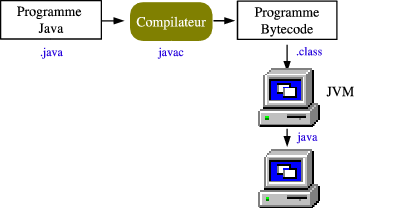
\includegraphics[width=0.8\linewidth,height=0.8\textheight,keepaspectratio=true]{/home/clr/Documents/Cours/DEV1Q2/TDSeq/fr/image/java-jvm-jvm.png}
						\end{center}
                
                    \caption[java-jvm-jvm.png]{java-jvm-jvm.png}
                \end{figure}
                    
            \par
        
          Prenons un exemple (fichier\verb@ Hello . java@)
          
            \par
        \begin{Java}
// Mon premier programme
public class Hello {
    public static void main(String [] args) {
        System.out. println ("Bonjour !");
    }
}
        \end{Java}
					\begin{itemize}
				
			\item Compilons-le \,\verb|javac Hello.java|\,
			\item On obtient la version compil\'ee, le bytecode (\verb@Hello . class@ )
			\item On peut l'ex\'ecuter \,\verb|java Hello|\,
			\item On voit alors apparaitre \`a l'\'ecran \verb@Bonjour !@
					\end{itemize}
				
            \par
        \section{Exercices}
				Maintenant, mettons tout \c ca en pratique.
      
            \par
        \subsection{Compr\'ehension d'algorithme}
          Pour ces exercices, nous vous demandons de comprendre des algorithmes donn\'es. 
          
			
		\subparagraph{Compr\'ehension} 
		
                \textcolor{white}{.} \par
            
							  Que vont-ils afficher si \`a chaque fois les deux nombres lus au d\'epart sont successivement 2 et 3 ?
							
					\begin{itemize}
				
			\item \begin{verbatim}
module exerciceA()
  lire a, b
  b ← b+2*a
  afficher b
fin module
				\end{verbatim} \textcolor{gray}{\underline{\hspace*{1em}}} 
			\item \begin{verbatim}
module exerciceB()
  a,b : entiers
  lire a, b
  a ← a+2*b
  afficher a
fin module
				\end{verbatim} \textcolor{gray}{\underline{\hspace*{1em}}} 
			\item \begin{verbatim}
module exerciceC()
  a,b : entiers
  lire b, a
  b ← b+2*a
  afficher b
fin module
				\end{verbatim} \textcolor{gray}{\underline{\hspace*{1em}}} 
			\item \begin{verbatim}
module exerciceD()
  a,b : entiers
  quotient : réel
  lire b, a
  quotient ← a / b
  afficher quotient
fin module
				\end{verbatim} \textcolor{gray}{\underline{\hspace*{2em}}} 
			\item \begin{verbatim}
module exerciceE()
  a, b, c, d : entiers
  lire c, d
  a ← 2*c+5*d
  b ← 2+c*3+d
  c ← a MOD b
  afficher a DIV c
fin module
				\end{verbatim} \textcolor{gray}{\underline{\hspace*{1em}}} 
			\item \begin{verbatim}
module exerciceF()
  x, y : réels
  lire x, y
  x ← x*x 
  x ← x*x+y*y 
  x ← √x
  afficher x
fin module
				\end{verbatim} \textcolor{gray}{\underline{\hspace*{1em}}} 
			\item \begin{verbatim}
module exerciceG()
  x, y : réels
  lire x, x
  x ← x MOD x + (x + 1) DIV 2
  afficher x + 3
fin module
				\end{verbatim} \textcolor{gray}{\underline{\hspace*{1em}}} 
					\end{itemize}
				
            \par
        \subsection{Compr\'ehension de codes Java}
          Pour ces exercices, nous vous demandons de comprendre des codes Java donn\'es. 
          
			
		\subparagraph{Compr\'ehension} 
		
                \textcolor{white}{.} \par
            
							  Que vont-ils afficher si \`a chaque fois les deux nombres lus au d\'epart sont successivement 2 et 3 ?
							
					\begin{itemize}
				
			\item \begin{Java}
import java.util.Scanner;
public class Exercice1 {
    public static void main(String [] args) {
        Scanner clavier = new Scanner(System.in);
        int nb1 = clavier.nextInt();
        int nb2 = clavier.nextInt();
        System.out.println(nb1 + " " + nb2);
    }
}
        \end{Java} \textcolor{gray}{\underline{\hspace*{2em}}} 
			\item \begin{Java}
import java.util.Scanner;
public class Exercice2 {
    public static void main(String [] args) {
        Scanner clavier = new Scanner(System.in);
        int nb1 = clavier.nextInt();
        int nb2 = clavier.nextInt();
        int nb3 = 2*nb1 + nb2;
        System.out.println(nb3);
    }
}
        \end{Java} \textcolor{gray}{\underline{\hspace*{1em}}} 
			\item \begin{Java}
import java.util.Scanner;
public class Exercice3 {
    public static void main(String [] args) {
        Scanner clavier = new Scanner(System.in);
        int nb2 = clavier.nextInt();
        int nb1 = clavier.nextInt();
        int nb3 = 2*nb1 + nb2;
        System.out.println(nb3);
    }
}
        \end{Java} \textcolor{gray}{\underline{\hspace*{1em}}} 
			\item \begin{Java}
import java.util.Scanner;
public class Exercice4 {
    public static void main(String [] args) {
        Scanner clavier = new Scanner(System.in);
        int nb1 = clavier.nextInt();
        int nb2 = clavier.nextInt();
        System.out.println(2*nb1 + nb2);
    }
}
        \end{Java} \textcolor{gray}{\underline{\hspace*{1em}}} 
			\item \begin{Java}
import java.util.Scanner;
public class Exercice5 {
    public static void main(String [] args) {
        Scanner clavier = new Scanner(System.in);
        int nb1 = clavier.nextInt();
        int nb2 = clavier.nextInt();
        System.out.println(nb2/nb1);
    }
}
        \end{Java} \textcolor{gray}{\underline{\hspace*{1em}}} 
			\item \begin{Java}
import java.util.Scanner;
public class Exercice6 {
    public static void main(String [] args) {
        Scanner clavier = new Scanner(System.in);
        int nb1 = clavier.nextInt();
        int nb2 = clavier.nextInt();
        System.out.println(nb1%nb2);
    }
}
        \end{Java} \textcolor{gray}{\underline{\hspace*{1em}}} 
			\item \begin{Java}
import java.util.Scanner;
public class Exercice7 {
    public static void main(String [] args) {
        Scanner clavier = new Scanner(System.in);
        int nb1 = clavier.nextInt();
        nb1 = clavier.nextInt();
        nb1 = nb1 * nb1;
        System.out.println(Math.sqrt(nb1));
    }
}
        \end{Java} \textcolor{gray}{\underline{\hspace*{1em}}} 
					\end{itemize}
				
            \par
        
			
		\subparagraph{Comprendre les erreurs} 
		
                \textcolor{white}{.} \par
            
								Soit le code :
							
            \par
        \begin{Java}
  public class ErrCompilation{
	  public static void main ( string[] args ) {
		  System.out.println("Hello !");
	  }
  }							\end{Java}
								la commande "\verb|javac ErrCompilation.java|"  provoque l'erreur suivante :
							
            \par
        \begin{verbatim}
  ErrCompilation.java:2:
  cannot find symbol
  symbol : class string
  location:class ErrCompilation
  public static void main ( string[] args ) {
  ^ 
  1
  error						\end{verbatim}
								Quelle est l'erreur ?
							
            \par
        
            \begin{itemize} 
        
            \item[ \ding{"6D} ] il faut ins\'erer des espaces dans la parenth\`ese
        
            \item[ \ding{"6D} ] string doit \^etre \'ecrit avec une majuscule au d\'ebut
        
            \item[ \ding{"6D} ] le fichier doit s'appeler string.java
        
            \item[ \ding{"6D} ] il faut remplacer les parenth\`eses par des accolades
        
            \end{itemize} 
        
			
		\subparagraph{Comprendre les erreurs} 
		
                \textcolor{white}{.} \par
            
								Soit le code :
							
            \par
        \begin{Java}
  public class ErrExecution {
      public void main ( String[] args ) {
          System.out.println(10);
      }
  }							\end{Java}
								la suite de commandes 
							
            \par
        \begin{verbatim}
  javac ErrExecution.java 
  java ErrExecution			\end{verbatim}
								provoque l'erreur suivante :
							
            \par
        \begin{verbatim}
  Exception in thread "main" java.lang.NoSuchMethodError: main\end{verbatim}
								il s'agit d'une erreur g\'en\'er\'ee par la machine virtuelle java car :
							
            \par
        
            \begin{itemize} 
        
            \item[ \ding{"6D} ] la machine virtuelle est mal install\'ee
        
            \item[ \ding{"6D} ] le source n'a pas \'et\'e compil\'e
        
            \item[ \ding{"6D} ] l'ent\^ete de la m\'ethode main est incorrect
        
            \item[ \ding{"6D} ] on ex\'ecute la mauvaise classe
        
            \end{itemize} 
        
			
		\subparagraph{Comprendre les erreurs} 
		
                \textcolor{white}{.} \par
            
								Soit le code :
							
            \par
        \begin{Java}
  public class ErrExecution {
      public static void main ( String[] args ) {	
          System.out.println(10);
      }
  }							\end{Java}
								la suite de commandes 
							
            \par
        \begin{verbatim}
  javac ErrExecution.java 
  java ErrExecution.java	\end{verbatim}
								provoque l'erreur suivante :
							
            \par
        \begin{verbatim}
  Exception in thread "main" java.lang.NoClassDefFoundError: ErrExecution/java
  caused by: java.lang.ClassNotFoundException: ErrExecution.java
  [...]
  Could not find the main class: ErrExecution.java. Program will exit.	\end{verbatim}
								il s'agit d'une erreur g\'en\'er\'ee par la machine virtuelle java car :
							
            \par
        
            \begin{itemize} 
        
            \item[ \ding{"6D} ] la machine virtuelle est mal install\'ee
        
            \item[ \ding{"6D} ] l'ent\^ete de la m\'ethode main est incorrect
        
            \item[ \ding{"6D} ] on ex\'ecute la mauvaise classe
        
            \end{itemize} 
        \subsection{\`A vous de jouer...}
			
		\subparagraph{Consignes} 
		
					\textcolor{white}{.} \par
				
          Il est temps de se lancer et d'\'ecrire vos premiers modules et programmes Java correspondant. 
          Voici quelques conseils pour vous guider dans la r\'esolution de tels probl\`emes :
          
					\begin{itemize}
				
			\item il convient d'abord de bien comprendre le probl\`eme pos\'e ; assurez-vous qu'il est parfaitement sp\'ecifi\'e ;
			\item r\'esolvez le probl\`eme via quelques exemples pr\'ecis ;
			\item mettez en \'evidence les variables \textbf{\guillemotleft  donn\'ees \guillemotright }, les variables \textbf{\guillemotleft  r\'esultats \guillemotright } et les variables de travail ;
			\item n'h\'esitez pas \`a faire une \'ebauche de r\'esolution en fran\c cais avant d'\'elaborer l'algorithme d\'efinitif pseudo-cod\'e ;
			\item d\'eclarez ensuite les variables (et leur type) qui interviennent dans l'algorithme ; les noms des variables risquant de ne pas \^etre suffisamment explicites.
			\item \'Ecrivez la partie algorithmique \textbf{AVANT} de vous lancer dans la programmation en Java.
					\end{itemize}
				
            \par
        
			
		\subparagraph{Exercice r\'esolu} 
		
					\textcolor{white}{.} \par
				
          La somme des angles d'un triangle est \'egale dans tous les cas \`a 180\textdegree . \'Ecrivez un algorithme qui lit la valeur de deux angles d'un triangle, et affiche la valeur du 3e. 
        
            \par
        
          Quelles sont les donn\'ees ? :
          
					\begin{enumerate}
				
			\item les 2 angles du triangle, ils sont lus au clavier.
					\end{enumerate}
				
          Que cherche-t-on ? :
          
					\begin{enumerate}
				
			\item la valeur du 3e angle du triangle, \`a afficher \`a l'\'ecran.
					\end{enumerate}
				
          Comment faire ? :
          
					\begin{enumerate}
				
			\item On sait que la somme des 3 angles d'un triangle vaut 180\textdegree . (angle1 + angle2 + angle3 = 180)
			\item On connait la valeur de 2 des angles, disons angle1 et angle2.
			\item La valeur du troisi\`eme angle vaut donc 180 moins la somme des 2 autres angles.(angle3 = 180 - (angle1 + angle2))
					\end{enumerate}
				
          \'Ecrivons l'algorithme :
          \begin{verbatim}
module troisièmeAngleTriangle()
    angle1, angle2, angle3 : réels
    lire angle1, angle2
    angle3 ← 180 - (angle1 + angle2)
    afficher angle3
fin module
          \end{verbatim}
          Traduisons cet algorithme en java :
          \begin{Java}
import java.util.Scanner;
public class Triangle{
    public static void main(String [] args) {
        Scanner clavier = new Scanner(System.in);
        double angle1 = clavier.nextDouble();
        double angle2 = clavier.nextDouble();
        double angle3 = 180 - (angle1 + angle2);
        System.out.println(angle3);
    }
}
        \end{Java}
        Il nous reste \`a compiler \,\verb|javac Triangle.java|\, et \`a ex\'ecuter \,\verb|java Triangle|\, notre programme.
        
            \par
        
			
		\subparagraph{\`A vous} 
		
					\textcolor{white}{.} \par
				
        \'Ecrivez les algorithmes et codez les programmes Java correspondant qui 
          
					\begin{enumerate}
				
			\item calcule et affiche la surface d'un carr\'e en lisant la valeur de son c\^ot\'e au clavier.
			\item calcule et affiche la surface d'un rectangle  en lisant les valeurs de sa longueur et sa largeur.
			\item calcule et affiche la surface d'un cercle en lisant la valeur de son rayon au clavier.  (Pensez \`a aller voir la classe Math pour obtenir la valeur de PI ;))
			\item \'etant donn\'e le prix unitaire d'un produit (hors TVA), le taux de TVA (en \%) 
            et la quantit\'e de produit vendue \`a un client, calcule et affiche le prix total \`a payer par ce client.
			\item r\'ealise la permutation du contenu de deux variables.
			\item calcule la somme des chiffres d'un nombre entier de 3 chiffres. R\'eflexion : l'algorithme est-il aussi valide pour les entiers inf\'erieurs \`a 100 ?
			\item \'etant donn\'e un moment dans la journ\'ee donn\'e par trois nombres lus, \`a savoir, heure, minute et seconde, calcule le nombre de secondes \'ecoul\'ees depuis minuit.
			\item \'etant donn\'e un temps \'ecoul\'e dans la journ\'ee exprim\'e en secondes, calcule et affiche ce temps sous la forme de trois nombres (heure, minute et seconde). \par
				
            Ex : 10000 secondes donnera 2h 46'40”
					\end{enumerate}
				
            \par
        
				\end{document}
			